\PassOptionsToPackage{dvipsnames,table}{xcolor}
\documentclass[11pt,a4paper]{article}

\usepackage{DS}

\begin{document}
\input{\detokenize{/home/fenarius/Travail/Cours/cpge-info/latex/Macros.tex}}
\ModeExercice
\DS{PC}{1}{Septembre 2023}
\newcommand{\SPATH}{/home/fenarius/Travail/Cours/cpge-info/docs/itc/Evaluations/DS/DS1}

\alertbox{\danger}{Consignes}{
	\begin{itemize}
		\item[\textbullet] On pourra toujours librement utiliser une fonction demandée à une question précédente même si cette question n'a pas été traitée.
		\item[\textbullet] Veillez à présenter vos idées et vos réponses partielles même si vous ne trouvez pas la solution complète à une question.
		\item[\textbullet] La clarté et la lisibilité de la rédaction et des programmes sont des éléments de notation.
	\end{itemize}
}

\begin{Exercise}[title = {Question de cours}] \\
	On considère la fonction {\tt puissance} ci-dessous :
	\inputpartPython{\SPATH /puissance.py}{}{\small}{1}{8}
	\Question{Montrer que cette fonction est correcte en mettant en évidence un invariant de boucle (sa spécification est donnée en commentaire dans le code ci-dessus).}
	\Question{Ecrire une version récursive de cette fonction et prouver qu'elle termine.}
\end{Exercise}

\begin{Exercise}[title = {anagrammes}] \\
	Deux mots \textit{de même longueur} sont anagrammes l'un de l'autre lorsque l'un est formé en réarrangeant les lettres de l'autre. Par exemple :
	\begin{itemize}
		\item \textit{niche} et \textit{chien} sont des anagrammes.
		\item \textit{epele} et \textit{pelle}, ne sont pas des anagrammes, en effet bien qu'ils soient formés avec les mêmes lettres, la lettre \textit{l} ne figure qu'à un seul exemplaire dans \textit{epele} et il en faut deux pour écrire \textit{pelle}.
	\end{itemize}
	Le but de l'exercice est d'écrire une fonction {\tt anagrammes} qui prend en argument deux chaines de caractères et qui renvoie {\tt true} si ces deux chaines sont des anagrammes et {\tt false} sinon.

	\ExePart[name = Une approche récursive]
Dans cette partie, on utilise une approche récursive.
\Question{Ecrire une fonction {\tt supprime\_premier} qui prend en argument un caractère {\tt car} et une chaine {\tt chaine} et renvoie la chaine obtenue en supprimant la premier occurence de {\tt car} dans {\tt chaine}.\\ Par exemple {\tt supprime\_premier("c","niche")} renvoie {\tt "nihe"}. Si {\tt car} n'est pas dans chaine alors on renvoie {\tt chaine} sans modification.\\ Par exemple {\tt supprime\_premier("l","Python")} renvoie {\tt "Python"}}
\Question{Ecrire une fonction récursive {\tt anagrammes\_rec} qui prend en argument deux chaines de caractères et renvoie {\tt True} si ce sont des anagrammes l'une de l'autre et {\tt False} sinon.\\ Par exemple, {\tt anagrammes\_rec("niche","chien")} renvoie {\tt True}.}
\Question{Donner (en la justifiant) la complexité de cette fonction en notant $n$ la taille de la plus longue des deux chaines.}

	\ExePart[name = Une approche itérative]
	Dans cette partie, on utilise une approche itérative en manipulant les dictionnaires de Python.
\Question{Ecrire une fonction {\tt cree\_dico} qui prend en argument une chaine de caractères et renvoie un dictionnaire dont les clés sont les caractères composant la chaine et les valeurs leur nombre d'apparition.\\ Par exemple, {\tt cree\_dico("epele")} renvoie le dictionnaire {\tt \{'e':3, 'p':1, 'l':1 \}} en effet dans le mot {\tt 'epele'}, {\tt 'e'} apparaît à trois reprises et {\tt 'l'} et {\tt 'p'} chacun une fois.}
\Question{Ecrire une fontionc {\tt egaux} qui prend en argument deux dictionnaires et renvoie {\tt True} si ces deux dictionnaires sont égaux (c'est-à-dire contiennent exactement les mêmes clés avec les mêmes valeurs) et {\tt False} sinon.\\ Par exemple, {\tt egaux(\{'e':3, 'p':1, 'l':1 \},\{'p':1,'e':2,'l':2\})} renvoie {\tt False}\\
\danger \; on s'interdit ici d'utiliser le test d'égalité {\tt ==} entre deux dictionnaires et on écrira un parcours de dictionnaire.
}
\Question{Ecrire une fonction {\tt anagrammes\_iter} qui prend en argument deux chaines de caractères et renvoie {\tt True} si ce sont des anagrammes et {\tt False} sinon.}
\Question{Donner (en la justifiant) la complexité de cette fonction en notant $n$ la taille de la plus longue des deux chaines.}

	

\end{Exercise}


\begin{Exercise}[title = {gestion de tests dans une entreprise},origin={\bac \; d'après {\sc ccinp 2023 - tpc, tsi}}] \\
\ExePart[name = Tests de code de sécurité sociale]
En France, le numéro de sécurité sociale se compose de 15 chiffres, comme détaillé sur l'image ci-dessous, les deux derniers chiffres sont calculés à partir des 13 premiers et forment une clé de contrôle destinée à vérifier que le numéro est valide. Le but de l'exercice est d'écrire un programme Python effectuant cette vérification.
\begin{center}
	\renewcommand{\arraystretch}{0.3}
	\begin{tabular}{r}
		\ \\
	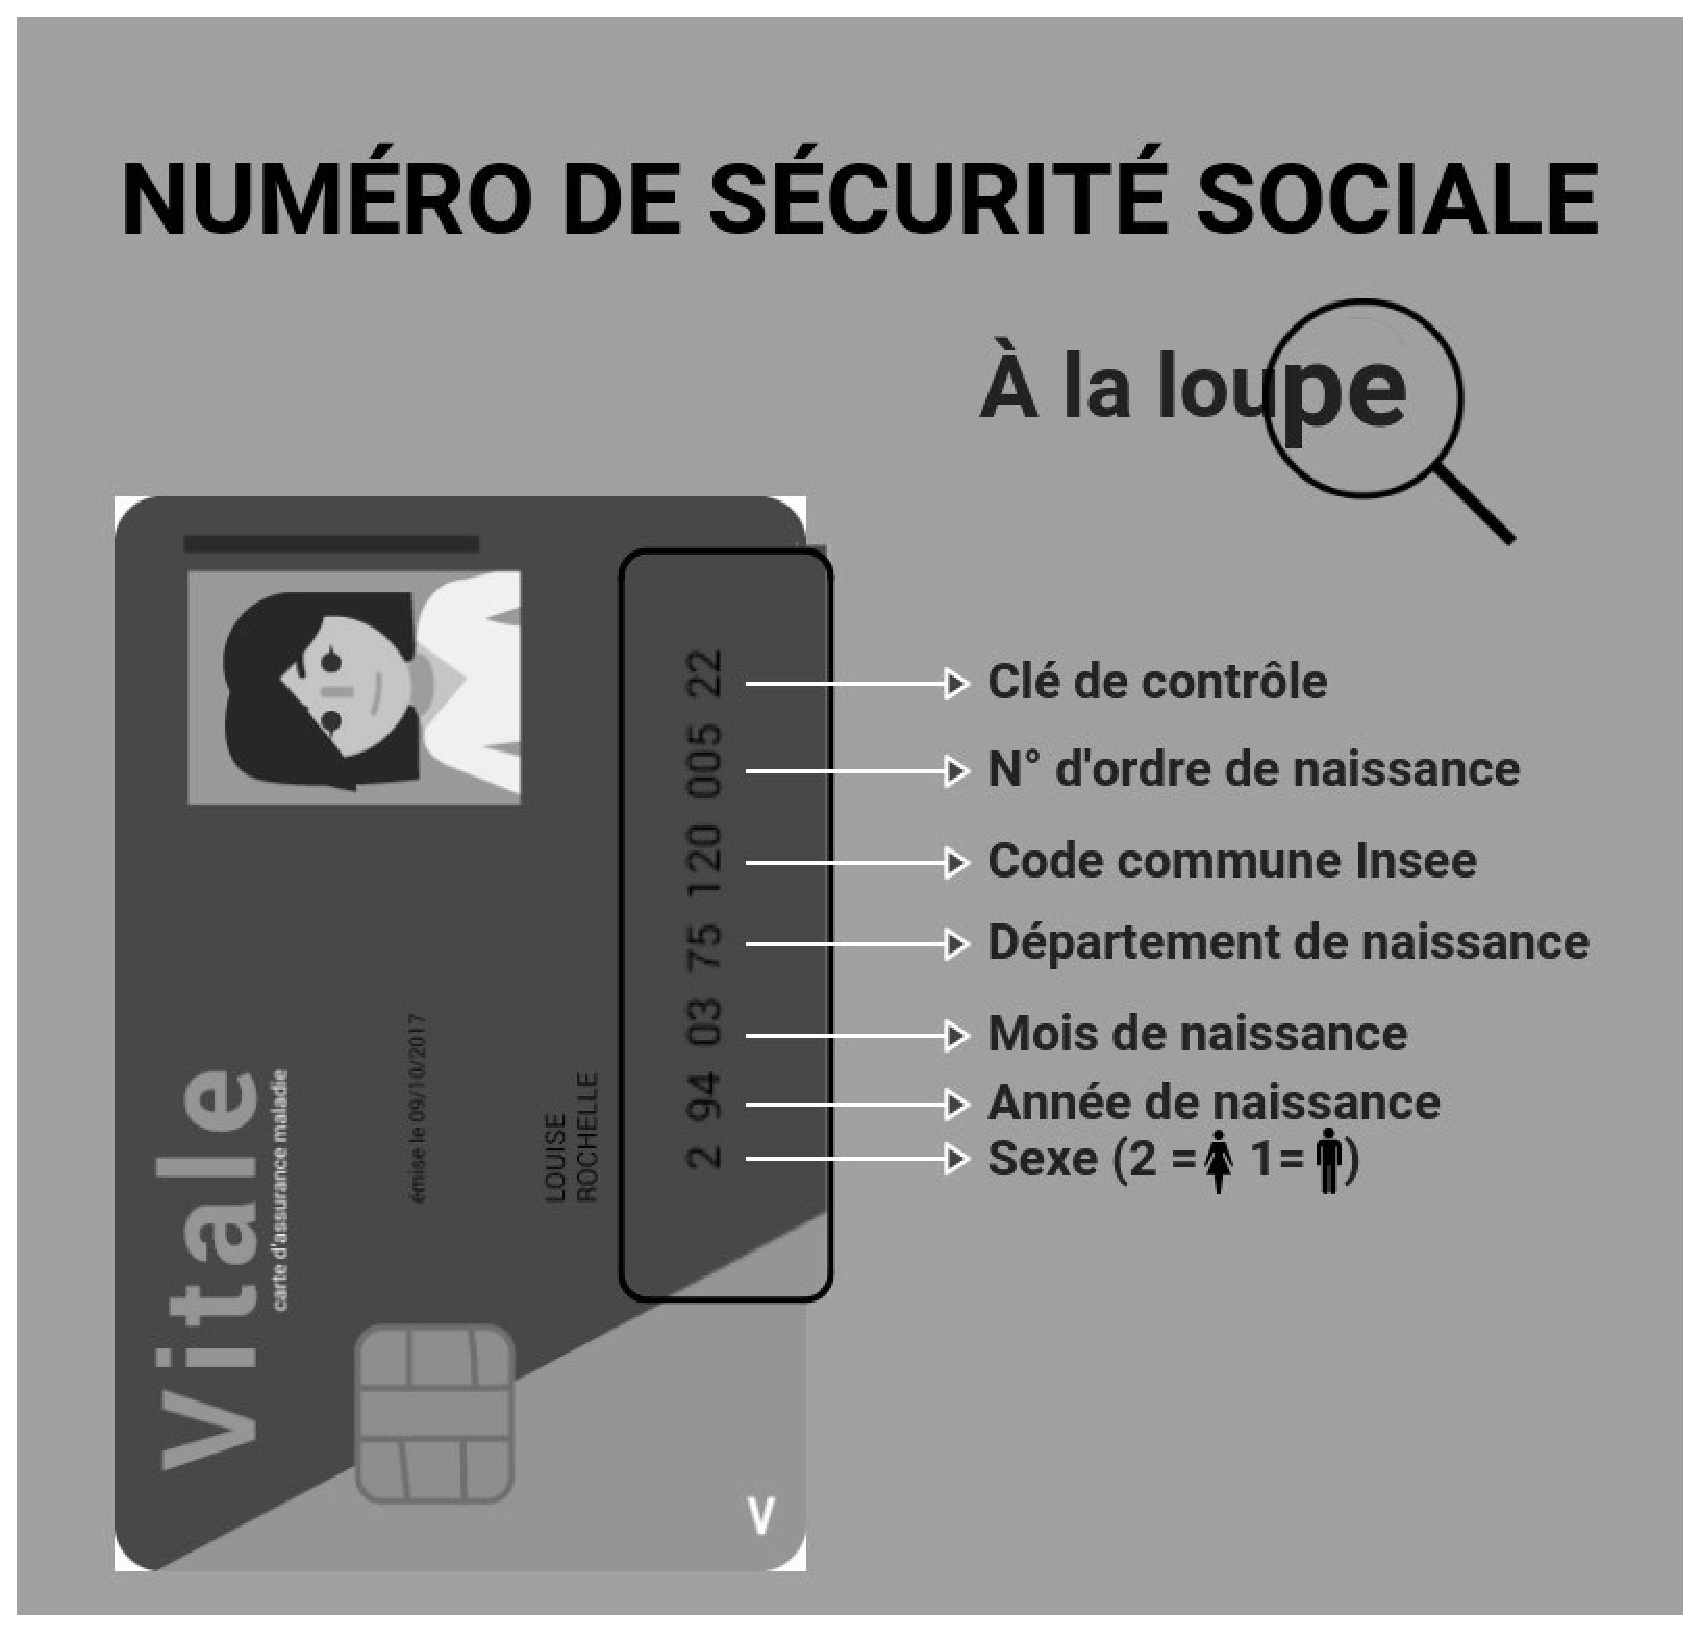
\includegraphics[width=10cm]{nss.eps} \\
	Credits : {\tt service-public.fr}\\
	\end{tabular}
\end{center}
Pour calculer la valeur de la clé de contrôle :
\begin{itemize}
	\item on calcule le reste dans la division euclidienne du nombre formé par les 13 premiers chiffres par 97,
	\item On soustrait de 97 le résultat obtenu.
\end{itemize}
Par exemple pour le numéro figurant sur l'image ci-dessus :
\begin{itemize}
	\item on calcule le reste dans la division euclidienne de $2\;94\;03\;75\;120\;005$ (les 13 premiers chiffres), on trouve~6.
	\item On soustrait de 97 le résultat obtenu : 97 - 6 = 91.
\end{itemize}
La clé de contrôle est dans ce cas 91, et donc le numéro ci-dessus est non valide puisque sa clé de contrôle est 22.

On suppose que les numéros de sécurité sociale sont fournis sous la forme de chaines de caractères (type  \textit{str} de Python) contenant des chiffres et des espaces, par exemple le numéro complet ci-dessous est donné sous la forme de la chaine {\tt "2 94 03 75 120 005 22"} et le numéro sans la clé de contrôle par {\tt "2 94 03 75 120 005"}. Et on rappelle qu'en Python, on peut toujours convertir une chaine de caractères en entier  (type \textit{int}) et inversement.

\Question{Ecrire la fonction {\tt num\_secu} qui prend en argument une chaine de caractères représentant un numéro de sécurité sociale (avec ou sans la clé), supprime les espaces  et renvoie le nombre entier formé par les chiffres de ce numéro de sécurité sociale. \\
Par exemple {\tt num\_secu("2 94 03 75 120 005")} renvoie l'entier {\tt 2940375120005}}
\Question{Ecrire la fonction {\tt clef} qui détermine la clé de contrôle d'un numéro de sécurité sociale à 13 chiffres. Cette fonction prend donc un paramètre de type {\tt int} et renvoie un {\tt int}.\\ 
Par exemple {\tt clef(2940375120005)} renvoie l'entier {\tt 91}}
\Question{Ecrire la fonction {\tt num\_secu\_complet} qui détermine le numéro de sécurité sociale complet à partir des 13 premiers chiffres. Cette fonction doit donc calculer la clé de contrôle et l'ajouter à la fin du numéro de sécurité social donné en argument. \\ Par exemple {\tt num\_secu\_complet(2940375120005)} renvoie l'entier {\tt 294037512000591} }
\Question{Ecrire la fonction {\tt test\_num\_secu} qui détermine si le numéro de sécurité social complet donné en argument (sous la forme d'une chaine de caractères) est correct. \\ Par exemple, {\tt test\_num\_secu("2 94 03 75 120 005 22")} renvoie {\tt False}.}
\ExePart[name = Tests de numéro de carte de crédit]
Comme pour les numéros de sécurité de sociale, un algorithme (appelé algorithme de Luhn), permet de vérifier qu'un numéro de carte de crédit est valide. Les étapes sont les suivantes :
\begin{itemize}
	\item on commence par extraire du numéro la liste des chiffres de rang impair ainsi que celle des chiffres de rang pair, en numérotant les chiffre à partir de la droite. Par exemple, sur le numéro {\tt 437716} cette procédure donne {\tt [3, 7, 6]} pour les chiffres de rang impair et {\tt [1, 7, 4]} pour ceux de rang pair. 
	\item On double ensuite chaque chiffre de la liste des rangs pairs et si on obtient un chiffre plus grand que 9, alors on le remplace par la somme des deux chiffres qui le compose. Dans l'exemple précédent, la liste des chiffres de rang pair {\tt [1, 7, 4]} devient donc {\tt [2, 5, 8]} car {\tt 14} est remplacé par la somme de ses chiffres donc 5.
	\item On calcule ensuite la somme des chiffres des deux listes, si le résultat obtenu est divisible par 10 alors le numéro de la carte de crédit est valide. Dans l'exemple précédent, on calcule donc :: \\ {\tt 3 + 7 + 6 + 2 + 5 + 8 = 33},\\ et comme 33 n'est pas divisible par 33, le numéro n'est pas valide.
\end{itemize}
\Question{Vérifier que le numéro {\tt 4762} est valide.}
\Question{Ecrire une fonction {\tt num\_en\_liste} qui prend en argument un entier et renvoie la liste de ses chiffres. Par exemple, 
{\tt num\_en\_liste(4762)} renvoie la liste {\tt [4, 7, 6, 2]}.}
\Question{Ecrire une fonction {\tt impairs\_pairs} qui prend en argument une liste {\tt l} et renvoie deux listes, celles des éléments d'indice impair de {\tt l} et celle  éléments d'indice pairs en numérotant les indices à partir de la droite. Par exemple {\tt pairs\_impairs([4, 7, 6, 2])} renvoie {\tt [2, 7]} et {\tt [6, 4]}}
\Question{Ecrire une fonction {\tt traite\_pairs} qui prend en argument une liste {\tt l}, ne renvoie rien et modifie cette liste en remplaçant chaque chiffre de la liste par son double. Si le résultat obtenu est supérieur à 9 alors il faut le remplacer par la somme des deux chiffres qui le composent. Par exemple, si  {\tt l=[6, 4]}, après l'appel {\tt traite\_pairs[l]}, le contenu de {\tt l} devient {\tt [3, 8]} en effet {\tt 4} a été remplacé par son double {\tt 8} et {\tt 6} par la somme des chiffres de son double {\tt 12}.}
\Question{Ecrire une fonction {\tt test\_num\_carte} qui prend en argument un entier et renvoie {\tt True} si c'est le numéro d'une carte de crédit valide et {\tt False} sinon. Par exemple, {\tt test\_num\_carte(4762)} renvoie {\tt True}}.
\end{Exercise}

\begin{Exercise}[title={requête {\sc sql} sur une seule table}]\\
	On considère la base de données {\tt pays\_du\_monde} contenant une seule table {\tt pays} dont le schéma est donné ci-dessous :
	\begin{center}
	\begin{tabular}{|lll|}
		\hline
		\multicolumn{3}{|c|}{\textbf{pays}} \\
		\hline
		{\tt nom} & : & {\sc text} \\
		\hline
		{\tt region} & : & {\sc text} \\
		\hline
		{\tt population} & : & {\sc int} \\
		\hline
		{\tt surface} & : & {\sc int} \\
		\hline
		{\tt cotes} & : & {\sc int} \\
		\hline
		{\tt pib} & : & {\sc int} \\
		\hline
		\end{tabular}
	\end{center}
	D'autre part, on précise la signification des champs suivants : 
	\begin{itemize}
		\item {\tt population} : le nombre d'habitants du pays.
		\item {\tt region} : La région du pays (par exemple "europe de l'ouest")
		\item {\tt area} : la surface du pays (en km carré).
		\item {\tt coastline} : la surface côtière du pays, cette valeur vaut 0 lorsque le pays n'a pas d'ouverture sur la mer
		\item {\tt pib} : le produit intérieur brut par habitant, c'est une mesure de la richesse du pays.
		\end{itemize}
	Et on indique que la requête \mintinline{sql}{SELECT DISTINCT region FROM pays} a renvoyé le résultat suivant : 
	\begin{center}
	\begin{tabular}{|l|}
		\hline
		\multicolumn{1}{|c|}{\textbf{region}} \\
		\hline
		Asie \\
		Afrique du nord \\
		Europe de l'est \\
		Europe de l'ouest \\
		Oceanie \\
		Afrique sub saharienne \\
		Proche orient\\
		Amérique latine\\
		Amérique du nord\\
		\hline
	\end{tabular}
\end{center}
Ecrire les requêtes permettant de :
\Question{Trouver la population et le produit intérieur brut de la France.}
\Question{Trouver les pays d'europe n'ayant pas d'ouverture sur la mer.}
\Question{Classer par ordre alphabétique les pays d'amérique latine.}
\Question{Lister par ordre décroissant du nombre d'habitants les cinq pays les plus peuplés}
\Question{Trouver le pays du proche orient le plus riche (ayant le {\tt pib} le plus élevé). }
\Question{Classer le pays d'afrique du nord par densité décroissante de population (la densité est le rapport entre le nombre d'habitant et la surface)}
\Question{Classer les régions par somme du pib décroissante des pays qui les composent.}



\end{Exercise}

	
\end{document}